% Created by tikzDevice version 0.12.3.1 on 2022-06-27 14:20:09
% !TEX encoding = UTF-8 Unicode
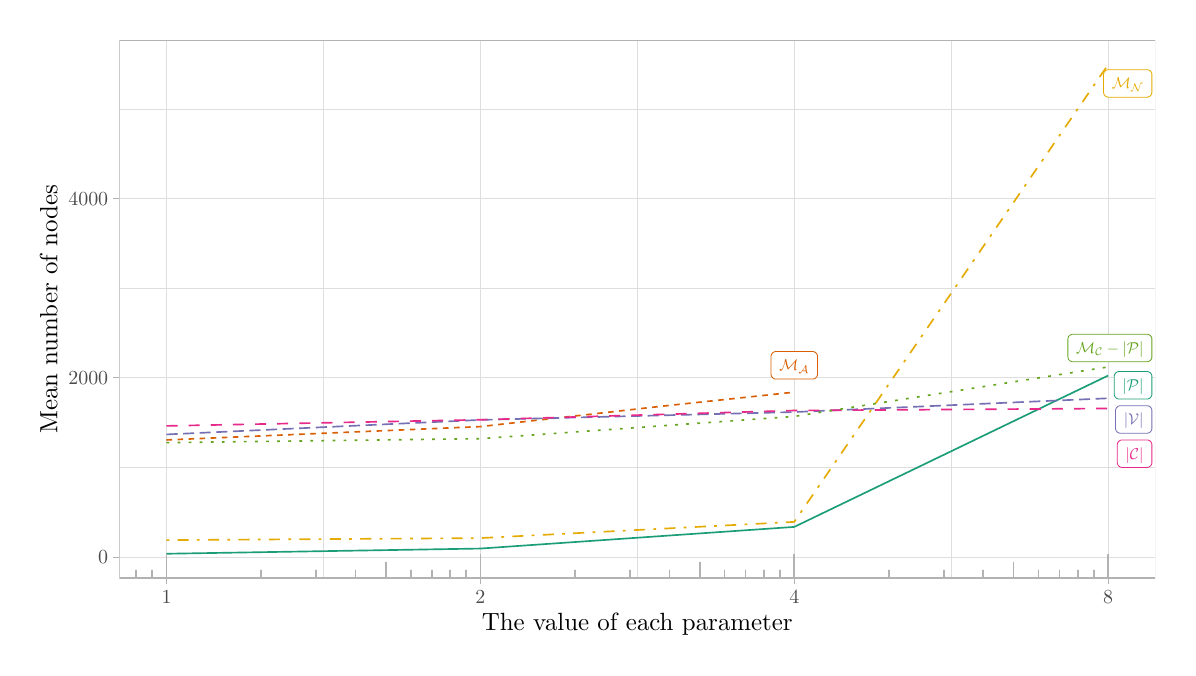
\begin{tikzpicture}[x=1pt,y=1pt]
\definecolor{fillColor}{RGB}{255,255,255}
\path[use as bounding box,fill=fillColor,fill opacity=0.00] (0,0) rectangle (411.94,224.04);
\begin{scope}
\path[clip] (  0.00,  0.00) rectangle (411.94,224.04);
\definecolor{drawColor}{RGB}{255,255,255}
\definecolor{fillColor}{RGB}{255,255,255}

\path[draw=drawColor,line width= 0.5pt,line join=round,line cap=round,fill=fillColor] (  0.00,  0.00) rectangle (411.94,224.04);
\end{scope}
\begin{scope}
\path[clip] ( 33.14, 25.11) rectangle (407.44,219.54);
\definecolor{fillColor}{RGB}{255,255,255}

\path[fill=fillColor] ( 33.14, 25.11) rectangle (407.44,219.54);
\definecolor{drawColor}{gray}{0.87}

\path[draw=drawColor,line width= 0.1pt,line join=round] ( 33.14, 65.17) --
	(407.44, 65.17);

\path[draw=drawColor,line width= 0.1pt,line join=round] ( 33.14,129.92) --
	(407.44,129.92);

\path[draw=drawColor,line width= 0.1pt,line join=round] ( 33.14,194.66) --
	(407.44,194.66);

\path[draw=drawColor,line width= 0.1pt,line join=round] (106.87, 25.11) --
	(106.87,219.54);

\path[draw=drawColor,line width= 0.1pt,line join=round] (220.29, 25.11) --
	(220.29,219.54);

\path[draw=drawColor,line width= 0.1pt,line join=round] (333.71, 25.11) --
	(333.71,219.54);

\path[draw=drawColor,line width= 0.2pt,line join=round] ( 33.14, 32.80) --
	(407.44, 32.80);

\path[draw=drawColor,line width= 0.2pt,line join=round] ( 33.14, 97.54) --
	(407.44, 97.54);

\path[draw=drawColor,line width= 0.2pt,line join=round] ( 33.14,162.29) --
	(407.44,162.29);

\path[draw=drawColor,line width= 0.2pt,line join=round] ( 50.16, 25.11) --
	( 50.16,219.54);

\path[draw=drawColor,line width= 0.2pt,line join=round] (163.58, 25.11) --
	(163.58,219.54);

\path[draw=drawColor,line width= 0.2pt,line join=round] (277.00, 25.11) --
	(277.00,219.54);

\path[draw=drawColor,line width= 0.2pt,line join=round] (390.43, 25.11) --
	(390.43,219.54);
\definecolor{drawColor}{RGB}{27,158,119}

\path[draw=drawColor,line width= 0.6pt,line join=round] ( 50.16, 33.94) --
	(163.58, 35.82) --
	(277.00, 43.64) --
	(390.43, 98.33);
\definecolor{drawColor}{RGB}{217,95,2}

\path[draw=drawColor,line width= 0.6pt,dash pattern=on 2pt off 2pt ,line join=round] ( 50.16, 75.06) --
	(163.58, 79.89) --
	(229.93, 87.34) --
	(277.00, 92.33);
\definecolor{drawColor}{RGB}{117,112,179}

\path[draw=drawColor,line width= 0.6pt,dash pattern=on 4pt off 2pt ,line join=round] ( 50.16, 77.05) --
	(163.58, 82.31) --
	(277.00, 85.14) --
	(390.43, 90.12);
\definecolor{drawColor}{RGB}{231,41,138}

\path[draw=drawColor,line width= 0.6pt,dash pattern=on 4pt off 4pt ,line join=round] ( 50.16, 80.14) --
	(163.58, 82.36) --
	(277.00, 85.70) --
	(390.43, 86.43);
\definecolor{drawColor}{RGB}{102,166,30}

\path[draw=drawColor,line width= 0.6pt,dash pattern=on 1pt off 3pt ,line join=round] ( 50.16, 74.09) --
	(163.58, 75.52) --
	(277.00, 83.56) --
	(390.43,101.45);
\definecolor{drawColor}{RGB}{230,171,2}

\path[draw=drawColor,line width= 0.6pt,dash pattern=on 1pt off 3pt on 4pt off 3pt ,line join=round] ( 50.16, 38.87) --
	(163.58, 39.60) --
	(277.00, 45.46) --
	(390.43,210.70);
\end{scope}
\begin{scope}
\path[clip] ( 33.14, 25.11) rectangle (407.44,219.54);

\path[] (399.52, 75.07) -- (390.90, 85.83);
\definecolor{drawColor}{RGB}{27,158,119}
\definecolor{fillColor}{RGB}{255,255,255}

\path[draw=drawColor,line width= 0.3pt,line join=round,line cap=round,fill=fillColor] (394.43, 89.84) --
	(404.43, 89.84) --
	(404.35, 89.85) --
	(404.65, 89.86) --
	(404.93, 89.92) --
	(405.20, 90.02) --
	(405.45, 90.16) --
	(405.68, 90.35) --
	(405.87, 90.57) --
	(406.03, 90.81) --
	(406.14, 91.08) --
	(406.21, 91.36) --
	(406.23, 91.65) --
	(406.23, 91.65) --
	(406.23, 97.98) --
	(406.23, 97.98) --
	(406.21, 98.27) --
	(406.14, 98.55) --
	(406.03, 98.82) --
	(405.87, 99.06) --
	(405.68, 99.28) --
	(405.45, 99.47) --
	(405.20, 99.61) --
	(404.93, 99.71) --
	(404.65, 99.77) --
	(404.43, 99.79) --
	(394.43, 99.79) --
	(394.65, 99.77) --
	(394.36, 99.78) --
	(394.07, 99.75) --
	(393.79, 99.67) --
	(393.53, 99.54) --
	(393.29, 99.38) --
	(393.08, 99.18) --
	(392.90, 98.94) --
	(392.77, 98.69) --
	(392.68, 98.41) --
	(392.63, 98.12) --
	(392.62, 97.98) --
	(392.62, 91.65) --
	(392.63, 91.80) --
	(392.63, 91.51) --
	(392.68, 91.22) --
	(392.77, 90.94) --
	(392.90, 90.68) --
	(393.08, 90.45) --
	(393.29, 90.25) --
	(393.53, 90.09) --
	(393.79, 89.96) --
	(394.07, 89.88) --
	(394.36, 89.85) --
	cycle;
\end{scope}
\begin{scope}
\path[clip] ( 33.14, 25.11) rectangle (407.44,219.54);
\definecolor{drawColor}{RGB}{27,158,119}

\node[text=drawColor,anchor=base,inner sep=0pt, outer sep=0pt, scale=  0.57] at (399.43, 92.86) {$|\mathcal{P}|$};
\definecolor{drawColor}{RGB}{117,112,179}
\definecolor{fillColor}{RGB}{255,255,255}

\path[draw=drawColor,line width= 0.3pt,line join=round,line cap=round,fill=fillColor] (394.90, 77.50) --
	(404.43, 77.50) --
	(404.35, 77.50) --
	(404.65, 77.51) --
	(404.93, 77.57) --
	(405.20, 77.67) --
	(405.45, 77.82) --
	(405.68, 78.00) --
	(405.87, 78.22) --
	(406.03, 78.46) --
	(406.14, 78.73) --
	(406.21, 79.01) --
	(406.23, 79.30) --
	(406.23, 79.30) --
	(406.23, 85.63) --
	(406.23, 85.63) --
	(406.21, 85.92) --
	(406.14, 86.20) --
	(406.03, 86.47) --
	(405.87, 86.72) --
	(405.68, 86.94) --
	(405.45, 87.12) --
	(405.20, 87.26) --
	(404.93, 87.37) --
	(404.65, 87.43) --
	(404.43, 87.44) --
	(394.90, 87.44) --
	(395.12, 87.43) --
	(394.83, 87.44) --
	(394.54, 87.40) --
	(394.26, 87.32) --
	(394.00, 87.20) --
	(393.76, 87.03) --
	(393.55, 86.83) --
	(393.37, 86.60) --
	(393.24, 86.34) --
	(393.15, 86.06) --
	(393.10, 85.78) --
	(393.09, 85.63) --
	(393.09, 79.30) --
	(393.10, 79.45) --
	(393.10, 79.16) --
	(393.15, 78.87) --
	(393.24, 78.60) --
	(393.37, 78.34) --
	(393.55, 78.11) --
	(393.76, 77.90) --
	(394.00, 77.74) --
	(394.26, 77.61) --
	(394.54, 77.53) --
	(394.83, 77.50) --
	cycle;
\end{scope}
\begin{scope}
\path[clip] ( 33.14, 25.11) rectangle (407.44,219.54);
\definecolor{drawColor}{RGB}{117,112,179}

\node[text=drawColor,anchor=base,inner sep=0pt, outer sep=0pt, scale=  0.57] at (399.66, 80.51) {$|\mathcal{V}|$};
\definecolor{drawColor}{RGB}{231,41,138}
\definecolor{fillColor}{RGB}{255,255,255}

\path[draw=drawColor,line width= 0.3pt,line join=round,line cap=round,fill=fillColor] (395.53, 65.13) --
	(404.43, 65.13) --
	(404.35, 65.13) --
	(404.65, 65.14) --
	(404.93, 65.20) --
	(405.20, 65.30) --
	(405.45, 65.45) --
	(405.68, 65.63) --
	(405.87, 65.85) --
	(406.03, 66.09) --
	(406.14, 66.36) --
	(406.21, 66.64) --
	(406.23, 66.93) --
	(406.23, 66.93) --
	(406.23, 73.26) --
	(406.23, 73.26) --
	(406.21, 73.55) --
	(406.14, 73.83) --
	(406.03, 74.10) --
	(405.87, 74.35) --
	(405.68, 74.56) --
	(405.45, 74.75) --
	(405.20, 74.89) --
	(404.93, 75.00) --
	(404.65, 75.05) --
	(404.43, 75.07) --
	(395.53, 75.07) --
	(395.75, 75.05) --
	(395.46, 75.07) --
	(395.17, 75.03) --
	(394.89, 74.95) --
	(394.63, 74.83) --
	(394.39, 74.66) --
	(394.18, 74.46) --
	(394.00, 74.23) --
	(393.87, 73.97) --
	(393.77, 73.69) --
	(393.73, 73.41) --
	(393.72, 73.26) --
	(393.72, 66.93) --
	(393.73, 67.08) --
	(393.73, 66.79) --
	(393.77, 66.50) --
	(393.87, 66.22) --
	(394.00, 65.97) --
	(394.18, 65.73) --
	(394.39, 65.53) --
	(394.63, 65.37) --
	(394.89, 65.24) --
	(395.17, 65.16) --
	(395.46, 65.13) --
	cycle;
\end{scope}
\begin{scope}
\path[clip] ( 33.14, 25.11) rectangle (407.44,219.54);
\definecolor{drawColor}{RGB}{231,41,138}

\node[text=drawColor,anchor=base,inner sep=0pt, outer sep=0pt, scale=  0.57] at (399.98, 68.14) {$|\mathcal{C}|$};
\definecolor{drawColor}{RGB}{102,166,30}
\definecolor{fillColor}{RGB}{255,255,255}

\path[draw=drawColor,line width= 0.3pt,line join=round,line cap=round,fill=fillColor] (377.69,103.32) --
	(404.43,103.32) --
	(404.35,103.32) --
	(404.65,103.33) --
	(404.93,103.39) --
	(405.20,103.49) --
	(405.45,103.64) --
	(405.68,103.82) --
	(405.87,104.04) --
	(406.03,104.29) --
	(406.14,104.55) --
	(406.21,104.84) --
	(406.23,105.13) --
	(406.23,105.13) --
	(406.23,111.45) --
	(406.23,111.45) --
	(406.21,111.74) --
	(406.14,112.03) --
	(406.03,112.29) --
	(405.87,112.54) --
	(405.68,112.76) --
	(405.45,112.94) --
	(405.20,113.09) --
	(404.93,113.19) --
	(404.65,113.25) --
	(404.43,113.26) --
	(377.69,113.26) --
	(377.90,113.25) --
	(377.61,113.26) --
	(377.32,113.22) --
	(377.05,113.14) --
	(376.78,113.02) --
	(376.54,112.85) --
	(376.33,112.65) --
	(376.16,112.42) --
	(376.02,112.16) --
	(375.93,111.89) --
	(375.89,111.60) --
	(375.88,111.45) --
	(375.88,105.13) --
	(375.89,105.27) --
	(375.89,104.98) --
	(375.93,104.69) --
	(376.02,104.42) --
	(376.16,104.16) --
	(376.33,103.93) --
	(376.54,103.73) --
	(376.78,103.56) --
	(377.05,103.44) --
	(377.32,103.36) --
	(377.61,103.32) --
	cycle;
\end{scope}
\begin{scope}
\path[clip] ( 33.14, 25.11) rectangle (407.44,219.54);
\definecolor{drawColor}{RGB}{102,166,30}

\node[text=drawColor,anchor=base,inner sep=0pt, outer sep=0pt, scale=  0.57] at (391.06,106.33) {$\mathcal{M}_{\mathcal{C}}-|\mathcal{P}|$};
\definecolor{drawColor}{RGB}{230,171,2}
\definecolor{fillColor}{RGB}{255,255,255}

\path[draw=drawColor,line width= 0.3pt,line join=round,line cap=round,fill=fillColor] (390.57,198.92) --
	(404.43,198.92) --
	(404.35,198.92) --
	(404.65,198.94) --
	(404.93,198.99) --
	(405.20,199.10) --
	(405.45,199.24) --
	(405.68,199.43) --
	(405.87,199.64) --
	(406.03,199.89) --
	(406.14,200.16) --
	(406.21,200.44) --
	(406.23,200.73) --
	(406.23,200.73) --
	(406.23,207.06) --
	(406.23,207.06) --
	(406.21,207.35) --
	(406.14,207.63) --
	(406.03,207.90) --
	(405.87,208.14) --
	(405.68,208.36) --
	(405.45,208.54) --
	(405.20,208.69) --
	(404.93,208.79) --
	(404.65,208.85) --
	(404.43,208.86) --
	(390.57,208.86) --
	(390.79,208.85) --
	(390.50,208.86) --
	(390.21,208.83) --
	(389.93,208.75) --
	(389.67,208.62) --
	(389.43,208.46) --
	(389.22,208.26) --
	(389.05,208.02) --
	(388.91,207.77) --
	(388.82,207.49) --
	(388.77,207.20) --
	(388.77,207.06) --
	(388.77,200.73) --
	(388.77,200.87) --
	(388.77,200.58) --
	(388.82,200.30) --
	(388.91,200.02) --
	(389.05,199.76) --
	(389.22,199.53) --
	(389.43,199.33) --
	(389.67,199.16) --
	(389.93,199.04) --
	(390.21,198.96) --
	(390.50,198.92) --
	cycle;
\end{scope}
\begin{scope}
\path[clip] ( 33.14, 25.11) rectangle (407.44,219.54);
\definecolor{drawColor}{RGB}{230,171,2}

\node[text=drawColor,anchor=base,inner sep=0pt, outer sep=0pt, scale=  0.57] at (397.50,201.93) {$\mathcal{M}_{\mathcal{N}}$};
\end{scope}
\begin{scope}
\path[clip] ( 33.14, 25.11) rectangle (407.44,219.54);
\definecolor{drawColor}{RGB}{217,95,2}
\definecolor{fillColor}{RGB}{255,255,255}

\path[draw=drawColor,line width= 0.3pt,line join=round,line cap=round,fill=fillColor] (270.41, 97.07) --
	(283.59, 97.07) --
	(283.52, 97.07) --
	(283.81, 97.09) --
	(284.10, 97.14) --
	(284.37, 97.25) --
	(284.62, 97.39) --
	(284.85, 97.58) --
	(285.04, 97.79) --
	(285.19, 98.04) --
	(285.31, 98.31) --
	(285.38, 98.59) --
	(285.40, 98.88) --
	(285.40, 98.88) --
	(285.40,105.21) --
	(285.40,105.21) --
	(285.38,105.50) --
	(285.31,105.78) --
	(285.19,106.05) --
	(285.04,106.29) --
	(284.85,106.51) --
	(284.62,106.69) --
	(284.37,106.84) --
	(284.10,106.94) --
	(283.81,107.00) --
	(283.59,107.01) --
	(270.41,107.01) --
	(270.63,107.00) --
	(270.34,107.01) --
	(270.05,106.98) --
	(269.77,106.90) --
	(269.51,106.77) --
	(269.27,106.61) --
	(269.06,106.41) --
	(268.88,106.17) --
	(268.75,105.92) --
	(268.66,105.64) --
	(268.61,105.35) --
	(268.60,105.21) --
	(268.60, 98.88) --
	(268.61, 99.02) --
	(268.61, 98.73) --
	(268.66, 98.45) --
	(268.75, 98.17) --
	(268.88, 97.91) --
	(269.06, 97.68) --
	(269.27, 97.48) --
	(269.51, 97.31) --
	(269.77, 97.19) --
	(270.05, 97.11) --
	(270.34, 97.07) --
	cycle;
\end{scope}
\begin{scope}
\path[clip] ( 33.14, 25.11) rectangle (407.44,219.54);
\definecolor{drawColor}{RGB}{217,95,2}

\node[text=drawColor,anchor=base,inner sep=0pt, outer sep=0pt, scale=  0.57] at (277.00,100.08) {$\mathcal{M}_{\mathcal{A}}$};
\definecolor{drawColor}{gray}{0.70}

\path[draw=drawColor,line width= 0.6pt,line join=round,line cap=round] ( 39.17, 25.11) -- ( 39.17, 27.95);

\path[draw=drawColor,line width= 0.6pt,line join=round,line cap=round] ( 44.97, 25.11) -- ( 44.97, 27.95);

\path[draw=drawColor,line width= 0.6pt,line join=round,line cap=round] ( 50.16, 25.11) -- ( 50.16, 33.64);

\path[draw=drawColor,line width= 0.6pt,line join=round,line cap=round] ( 84.30, 25.11) -- ( 84.30, 27.95);

\path[draw=drawColor,line width= 0.6pt,line join=round,line cap=round] (104.27, 25.11) -- (104.27, 27.95);

\path[draw=drawColor,line width= 0.6pt,line join=round,line cap=round] (118.45, 25.11) -- (118.45, 27.95);

\path[draw=drawColor,line width= 0.6pt,line join=round,line cap=round] (129.44, 25.11) -- (129.44, 30.80);

\path[draw=drawColor,line width= 0.6pt,line join=round,line cap=round] (138.42, 25.11) -- (138.42, 27.95);

\path[draw=drawColor,line width= 0.6pt,line join=round,line cap=round] (146.01, 25.11) -- (146.01, 27.95);

\path[draw=drawColor,line width= 0.6pt,line join=round,line cap=round] (152.59, 25.11) -- (152.59, 27.95);

\path[draw=drawColor,line width= 0.6pt,line join=round,line cap=round] (158.39, 25.11) -- (158.39, 27.95);

\path[draw=drawColor,line width= 0.6pt,line join=round,line cap=round] (163.58, 25.11) -- (163.58, 33.64);

\path[draw=drawColor,line width= 0.6pt,line join=round,line cap=round] (197.72, 25.11) -- (197.72, 27.95);

\path[draw=drawColor,line width= 0.6pt,line join=round,line cap=round] (217.70, 25.11) -- (217.70, 27.95);

\path[draw=drawColor,line width= 0.6pt,line join=round,line cap=round] (231.87, 25.11) -- (231.87, 27.95);

\path[draw=drawColor,line width= 0.6pt,line join=round,line cap=round] (242.86, 25.11) -- (242.86, 30.80);

\path[draw=drawColor,line width= 0.6pt,line join=round,line cap=round] (251.84, 25.11) -- (251.84, 27.95);

\path[draw=drawColor,line width= 0.6pt,line join=round,line cap=round] (259.43, 25.11) -- (259.43, 27.95);

\path[draw=drawColor,line width= 0.6pt,line join=round,line cap=round] (266.01, 25.11) -- (266.01, 27.95);

\path[draw=drawColor,line width= 0.6pt,line join=round,line cap=round] (271.81, 25.11) -- (271.81, 27.95);

\path[draw=drawColor,line width= 0.6pt,line join=round,line cap=round] (277.00, 25.11) -- (277.00, 33.64);

\path[draw=drawColor,line width= 0.6pt,line join=round,line cap=round] (311.15, 25.11) -- (311.15, 27.95);

\path[draw=drawColor,line width= 0.6pt,line join=round,line cap=round] (331.12, 25.11) -- (331.12, 27.95);

\path[draw=drawColor,line width= 0.6pt,line join=round,line cap=round] (345.29, 25.11) -- (345.29, 27.95);

\path[draw=drawColor,line width= 0.6pt,line join=round,line cap=round] (356.28, 25.11) -- (356.28, 30.80);

\path[draw=drawColor,line width= 0.6pt,line join=round,line cap=round] (365.26, 25.11) -- (365.26, 27.95);

\path[draw=drawColor,line width= 0.6pt,line join=round,line cap=round] (372.86, 25.11) -- (372.86, 27.95);

\path[draw=drawColor,line width= 0.6pt,line join=round,line cap=round] (379.43, 25.11) -- (379.43, 27.95);

\path[draw=drawColor,line width= 0.6pt,line join=round,line cap=round] (385.24, 25.11) -- (385.24, 27.95);

\path[draw=drawColor,line width= 0.6pt,line join=round,line cap=round] (390.43, 25.11) -- (390.43, 33.64);

\path[draw=drawColor,line width= 0.5pt,line join=round,line cap=round] ( 33.14, 25.11) rectangle (407.44,219.54);
\end{scope}
\begin{scope}
\path[clip] (  0.00,  0.00) rectangle (411.94,224.04);
\definecolor{drawColor}{gray}{0.30}

\node[text=drawColor,anchor=base east,inner sep=0pt, outer sep=0pt, scale=  0.72] at ( 29.09, 30.32) {0};

\node[text=drawColor,anchor=base east,inner sep=0pt, outer sep=0pt, scale=  0.72] at ( 29.09, 95.06) {2000};

\node[text=drawColor,anchor=base east,inner sep=0pt, outer sep=0pt, scale=  0.72] at ( 29.09,159.81) {4000};
\end{scope}
\begin{scope}
\path[clip] (  0.00,  0.00) rectangle (411.94,224.04);
\definecolor{drawColor}{gray}{0.70}

\path[draw=drawColor,line width= 0.2pt,line join=round] ( 30.89, 32.80) --
	( 33.14, 32.80);

\path[draw=drawColor,line width= 0.2pt,line join=round] ( 30.89, 97.54) --
	( 33.14, 97.54);

\path[draw=drawColor,line width= 0.2pt,line join=round] ( 30.89,162.29) --
	( 33.14,162.29);
\end{scope}
\begin{scope}
\path[clip] (  0.00,  0.00) rectangle (411.94,224.04);
\definecolor{drawColor}{gray}{0.70}

\path[draw=drawColor,line width= 0.2pt,line join=round] ( 50.16, 22.86) --
	( 50.16, 25.11);

\path[draw=drawColor,line width= 0.2pt,line join=round] (163.58, 22.86) --
	(163.58, 25.11);

\path[draw=drawColor,line width= 0.2pt,line join=round] (277.00, 22.86) --
	(277.00, 25.11);

\path[draw=drawColor,line width= 0.2pt,line join=round] (390.43, 22.86) --
	(390.43, 25.11);
\end{scope}
\begin{scope}
\path[clip] (  0.00,  0.00) rectangle (411.94,224.04);
\definecolor{drawColor}{gray}{0.30}

\node[text=drawColor,anchor=base,inner sep=0pt, outer sep=0pt, scale=  0.72] at ( 50.16, 16.10) {1};

\node[text=drawColor,anchor=base,inner sep=0pt, outer sep=0pt, scale=  0.72] at (163.58, 16.10) {2};

\node[text=drawColor,anchor=base,inner sep=0pt, outer sep=0pt, scale=  0.72] at (277.00, 16.10) {4};

\node[text=drawColor,anchor=base,inner sep=0pt, outer sep=0pt, scale=  0.72] at (390.43, 16.10) {8};
\end{scope}
\begin{scope}
\path[clip] (  0.00,  0.00) rectangle (411.94,224.04);
\definecolor{drawColor}{RGB}{0,0,0}

\node[text=drawColor,anchor=base,inner sep=0pt, outer sep=0pt, scale=  0.90] at (220.29,  6.25) {The value of each parameter};
\end{scope}
\begin{scope}
\path[clip] (  0.00,  0.00) rectangle (411.94,224.04);
\definecolor{drawColor}{RGB}{0,0,0}

\node[text=drawColor,rotate= 90.00,anchor=base,inner sep=0pt, outer sep=0pt, scale=  0.90] at ( 10.70,122.32) {Mean number of nodes};
\end{scope}
\end{tikzpicture}
